%
% Modified by Megan Patnott
% Last Change: Jan 18, 2013
%
%%%%%%%%%%%%%%%%%%%%%%%%%%%%%%%%%%%%%%%%%%%%%%%%%%%%%%%%%%%%%%%%%%%%%%%%
%
% Modified by Sameer Vijay
% Last Change: Tue Jul 26 2005 13:00 CEST
%
%%%%%%%%%%%%%%%%%%%%%%%%%%%%%%%%%%%%%%%%%%%%%%%%%%%%%%%%%%%%%%%%%%%%%%%%
%
% Sample Notre Dame Thesis/Dissertation
% Using Donald Peterson's ndthesis classfile
%
% Written by Jeff Squyres and Don Peterson
%
% Provided by the Information Technology Committee of
%   the Graduate Student Union
%   http://www.gsu.nd.edu/
%
% Nothing in this document is serious except the format.  :-)
%
% If you have any suggestions, comments, questions, please send e-mail
% to: ndthesis@gsu.nd.edu
%
%%%%%%%%%%%%%%%%%%%%%%%%%%%%%%%%%%%%%%%%%%%%%%%%%%%%%%%%%%%%%%%%%%%%%%%%


%
% Chapter 5
%


\chapter{R-matrix analysis}
\label{chap: r-matrix}

An $R$-matrix analysis was performed to analyze the effects of the new lifetime and cross sections measurements described earlier. Such an analysis can be used to transform the cross sections into $S$-factors, which removes the Coulomb repulsion component of the cross-section and provides higher fidelity extrapolations to astrophysical energies. The $^{14}$N$(p,\gamma)^{15}$O system is ideal for $R$-matrix analysis because it is comprised of light nuclei with a discrete level structure at relatively low energies. While there are many programs available for performing $R$-matrix fits, we use the \texttt{AZURE2} code \cite{Azuma2010}, which was also used for similar, previous measurements \cite{Li2016}. 

\section{Impact of new lifetimes}
\label{sec: lifetime fit}

Following the analysis of \citet{Li2016}, the width of the 6.79 MeV state in $^{15}$O  was previously the largest source of uncertainty in the low-energy extrapolations of the cross section. A set of $R$-matrix fits was employed to explore the impact of our newly measured lifetimes. To isolate the effects of our measurement, we selected discrete lifetimes within our uncertainty range for the lifetime of the 6.79 MeV state in $^{15}$O, converted them to their equivalent radiative width, and used those level width values throughout the fit and extrapolation. This collection of fits, therefore, serves primarily as an illustration of the ways in which these new lifetime measurements impact the low energy extrapolations of the cross section.

In the fits presented here, the information about the levels was taken from  \citet{Ajzenberg-Selove1991} or \citet{Daigle2016} where updated. A channel radius of 5.5 fm was adopted for this work, which matches the analyses done by Refs.~\cite{Adelberger2011, Li2016, Wagner2018}. Information about the levels and their parameters as used in \texttt{AZURE2} are contained in Table~\ref{table: fitParams}. 


\begin{table*}[]
\thisfloatpagestyle{plain}
\caption{$R$-MATRIX FIT PARAMETERS FOR EXPLORING THE IMPACT OF NEWLY MEASURED LIFETIMES}
\begin{center}
\begin{threeparttable}
\begin{tabular}{c  c  c  c  c  c  c}
\toprule
$E_x$ (Ref.~\cite{Ajzenberg-Selove1991}) &   $E_x$ (fit) & $J^\pi$ & Channel & l & s & ANC (fm$^{-1/2}$) / $\Gamma$ (eV)\\ 
\midrule
0.0 & 0.0	& 1/2$^-$ &	$^{14}$N+p &	1&	1/2&	{0.23}\\
	&	&	    &    $^{14}$N+p &	1&	3/2&	{7.4} \\
%5.183(1) & \textbf{5.183}&	1/2$^+$&	$^{14}$N+p&	0&	1/2&	\textbf{0.33}\\
%	&	&		    &$^{15}$O+$\gamma_{0.00}$  &	E1&	1/2&	\textbf{0.0784}\\
%5.2409(3) & \textbf{5.2409}&	5/2$^+$&	$^{14}$N+p &	2&	1/2&	\textbf{0.23}\\
%                &	&		  & $^{14}$N+p &	2&	3/2&	\textbf{0.24}\\
%	 			&	&	 &$^{15}$O+$\gamma_{0.00}$	&M2&	1/2&	\textbf{0.0002}\\
%6.1763(17) & \textbf{6.1763}&	3/2$^-$& $^{14}$N+p &	1&	1/2&	\textbf{0.47}\\
%				&	&	& $^{14}$N+p	&1	&3/2	&\textbf{0.53}\\
%				&	&	&$^{15}$O+$\gamma_{0.00}$	&M1	&1/2&	\textbf{0.865}\\
6.7931(17) & {6.7931}&	3/2$^+$ & $^{14}$N+p &	0&	3/2&	{4.75}\\
	&	&	     &  $^{15}$O+$\gamma_{0.00}$	&  E1  &	1/2&	\textbf{2.50$^{\text{a}}$}\\
%	& &       &  $^{15}$O+$\gamma_{6.17}$	&  E1  &	3/2&{-0.002}\\
%6.8594(9) & \textbf{6.8594}&	5/2$^+$&	$^{14}$N+p&	2&	1/2&\textbf{0.39}\\
%	&		&    &     $^{14}$N+p&	2&	3/2&	\textbf{0.42}\\
%	&		&    &     $^{15}$O+$\gamma_{5.24}$&	M1&	5/2&	\textbf{0.04}\\
%7.2759(6) & \textbf{7.2759}&	7/2$^+$&	$^{14}$N+p &	2&	3/2&	\textbf{1541}\\
%	&		&    &     $^{15}$O+$\gamma_{5.24}$&	M1&	5/2&	\textbf{0.00099}\\
\hline
%7.5565(4) & 7.5563	&	1/2$^+$	&	$^{14}$N+p	&	0	&	1/2	&	\textbf{1.0$\times$10$^3$}	\\
%	&	&	&	$^{15}$O+$\gamma_{0.00}$	&	E1	&	1/2	&	\textbf{0.61$\times$10$^{-3}$}\\
%	&	&	&	$^{15}$O+$\gamma_{6.79}$	&	M1	&	3/2	&	\textbf{8.22$\times$10$^{-3}$}\\
%	&	&	&	$^{15}$O+$\gamma_{5.18}$	&	M1	&	1/2	&	\textbf{0.006}\\
%	&	&	&	$^{15}$O+$\gamma_{6.17}$	&	E1	&	3/2	&	\textbf{0.0254}\\
8.2840(5)& \textbf{8.2848}&	3/2$^+$	&	$^{14}$N+p	&	2	&	1/2	&	{-92.2}\\
	&	&	&	$^{14}$N+p	&	0	&	3/2	&	\textbf{4.013$\times$10$^3$}\\
	&	&	&	$^{14}$N+p	&	2	&	3/2	&	{-509}\\
	&	&	&	$^{15}$O+$\gamma_{0.00}$	&	E1	&	1/2	&	\textbf{0.244}\\
%	&	&	&	$^{15}$O+$\gamma_{5.18}$	&	M1	&	1/2	&	{0.01}\\
%	&	&	&	$^{15}$O+$\gamma_{5.24}$	&	M1	&	5/2	&	{0.2}\\
%	&	&	&	$^{15}$O+$\gamma_{6.17}$	&	E1	&	3/2	&	{-4$\times$10$^{-3}$}\\
%	&	&	&	$^{15}$O+$\gamma_{6.86}$	&	M1	&	5/2	&	{0.01}\\
%8.743(6) & \textbf{8.7502}&	1/2$^+$	&	$^{14}$N+p	&	0	&	1/2	&	\textbf{35.726$\times$10$^3$}\\
%	&	&	&	$^{15}$O+$\gamma_{5.18}$	&	M1	&	1/2	&	\textbf{-0.2}\\
%	&	&	&	$^{15}$O+$\gamma_{6.17}$	&	E1	&	3/2	&	\textbf{0.0827}\\
%8.922(2) & \textbf{8.9219}&	5/2$^+$	&	$^{14}$N+p	&	2	&	3/2	&	\textbf{3.8$\times$10$^3$}\\
%	&	&	&	$^{15}$O+$\gamma_{6.79}$	&	M1	&	3/2	&	\textbf{0.003}\\
8.9821(17) & {8.98}&	5/2$^-$	&	$^{14}$N+p	&	1	&	3/2	&	\textbf{-5.872$\times$10$^3$}\\
	&	&	&	$^{15}$O+$\gamma_{0.00}$	&	E2	&	1/2	&	\textbf{-0.303}\\
	&	&	&	$^{15}$O+$\gamma_{6.79}$	&	E1	&	3/2	&	{-0.001}\\
9.484(8) & \textbf{9.488}&	3/2$^+$	&	$^{14}$N+p	&	2	&	1/2	&	{77.69$\times$10$^3$}	\\
	&	&	&	$^{14}$N+p	&	0	&	3/2	&	\textbf{126.685$\times$10$^3$}	\\
	&	&	&	$^{14}$N+p	&	2	&	3/2	&	{-7.822$\times$10$^3$}\\
	&	&	&	$^{15}$O+$\gamma_{0.00}$	&	E1	&	1/2	&	\textbf{6.92}\\
%	&	&	&	$^{15}$O+$\gamma_{6.86}$	&	M1	&	5/2	&	{0.2}\\
9.488(3) & {9.4905}&	5/2$^-$	&	$^{14}$N+p	&	3	&	1/2	&	{0.979$\times$10$^3$}\\
	&	&	&	$^{14}$N+p	&	1	&	3/2	&	{-6.576$\times$10$^3$}\\
	&	&	&	$^{14}$N+p	&	3	&	3/2	&	{-0.985$\times$10$^3$}\\
	&	&	&	$^{15}$O+$\gamma_{0.00}$	&	E2	&	1/2	&	\textbf{-0.307}\\
	&	&	&	$^{15}$O+$\gamma_{6.79}$	&	E1	&	3/2	&	{-0.0123}\\
9.609(2) & {9.6075}&	3/2$^-$	&	$^{14}$N+p	&	1	&	3/2	&	\textbf{-13.821$\times$10$^3$}\\
	&	&	&	$^{15}$O+$\gamma_{0.00}$	&	M1	&	1/2	&	\textbf{1.24}\\
     &	&	&	$^{15}$O+$\gamma_{6.79}$	&	E1	&	3/2	&	{-0.044}\\
%	&	&	&	$^{15}$O+$\gamma_{5.24}$	&	E1	&	5/2	&	{0.095}\\
%10.2817 & \textbf{10.2817}	&	5/2$^+$	&	$^{14}$N+p	&	2	&	3/2	&	\textbf{17.292$\times$10$^3$}\\
%	&	&	&	$^{15}$O+$\gamma_{6.79}$	&	M1	&	3/2	&	\textbf{0.2}\\	
%	&	&	&	$^{15}$O+$\gamma_{6.86}$	&	M1	&	5/2	&	\textbf{-0.4}\\	
%10.480 & \textbf{10.4675}	&	3/2$^-$	&	$^{14}$N+p	&	1	&	1/2	&	\textbf{28.998$\times$10$^3$}\\
%	&	&	&	$^{14}$N+p	&	1	&	3/2	&	\textbf{9.652$\times$10$^3$}\\
%	&	&	&	$^{15}$O+$\gamma_{0.00}$	&	M1	&	1/2	&	\textbf{-0.404}\\	
%	&	&	&	$^{15}$O+$\gamma_{6.79}$	&	E1	&	3/2	&	\textbf{0.1}\\
%	&	&	&	$^{15}$O+$\gamma_{6.86}$	&	E1	&	5/2	&	\textbf{0.1}\\
%10.506 & \textbf{10.5313}&	3/2$^+$	&	$^{14}$N+p	&	0	&	3/2	&	\textbf{205$\times$10$^3$}\\
%	&	&	&	$^{15}$O+$\gamma_{0.00}$	&	E1	&	1/2	&	\textbf{-0.195}\\
%	&	&	&	$^{15}$O+$\gamma_{6.79}$	&	M1	&	3/2	&	\textbf{0.3}\\
%	&	&	&	$^{15}$O+$\gamma_{6.86}$	&	M1	&	5/2	&	\textbf{-0.4}\\
%10.9288 & \textbf{10.9288}&	7/2$^+$	&	$^{14}$N+p	&	2	&	3/2	&	\textbf{56.948$\times$10$^3$}\\
%	&	&	&	$^{15}$O+$\gamma_{6.79}$	&	E2&	3/2	&	\textbf{1}\\
%11.218(3) & 11.217(2)& 3/2$^+$&	$^{14}$N+p	&	0	&	3/2	&	\textbf{40$\times$10$^3$}\\
%	&	&	&	$^{15}$O+$\gamma_{0.00}$	&	E1	&	1/2	& 5.21	\\   	
& {15}	&	3/2$^+$	&	$^{14}$N+p	&	0	&	3/2	&	\textbf{4.722$\times$10$^6$}\\
	&	&	&	$^{15}$O+$\gamma_{0.00}$	&	E1	&	1/2	&	\textbf{327.3}	\\
%& \textbf{15}	&	5/2$^+$	&	$^{14}$N+p	&	2	&	1/2	&	\textbf{1.452$\times$10$^7$}\\
\bottomrule
\end{tabular}
\begin{tablenotes}
\small 
\item Levels used in the \textit{R}-matrix fits. Bold values indicate parameters which were allowed to vary during the fit. The signs on the partial widths and ANCs indicates the relative interferences. The dividing line demarcates the proton separation energy at $E_x$ = 7.2968(5) MeV \cite{Ajzenberg-Selove1991}. Levels where all parameters are fixed are not shown in this table for brevity but were included in the fits. a) Indicates the partial width of the 6.79 MeV state, measured in this experiment to between $\Gamma$ = 0.66 - 3.29 eV. For each individual fit, this width was fixed. However, between each fit, this width was varied to different values within our range to explore how the uncertainty in this measurement affects the low energy extrapolation. These different fits are shown in Fig.\ \ref{fig: rmatrixRange} and are otherwise identical.
\end{tablenotes}
\end{threeparttable}
\label{table: fitParams}
\end{center}
\end{table*}  



The cross-section data utilized in the fitting routine were from measurements at LUNA \cite{Formicola2004, Imbriani2005, Marta2008, Marta2011}, TUNL \cite{Runkle2005}, Bochum \cite{Schroder1987}, and the University of Notre Dame \cite{Li2016}. All of these data sets were left without scaling during the fits. The Bochum data from \citet{Schroder1987} were corrected as detailed in SFII \cite{Adelberger2011}. Additionally, the data used from \citet{Li2016} are a differential cross section taken at 45$\degree$ and are treated as such in the fits. This dataset was scaled by a factor of 4$\pi$ in the plotting only to compare to the angle integrated data. 



\begin{figure}[h!]
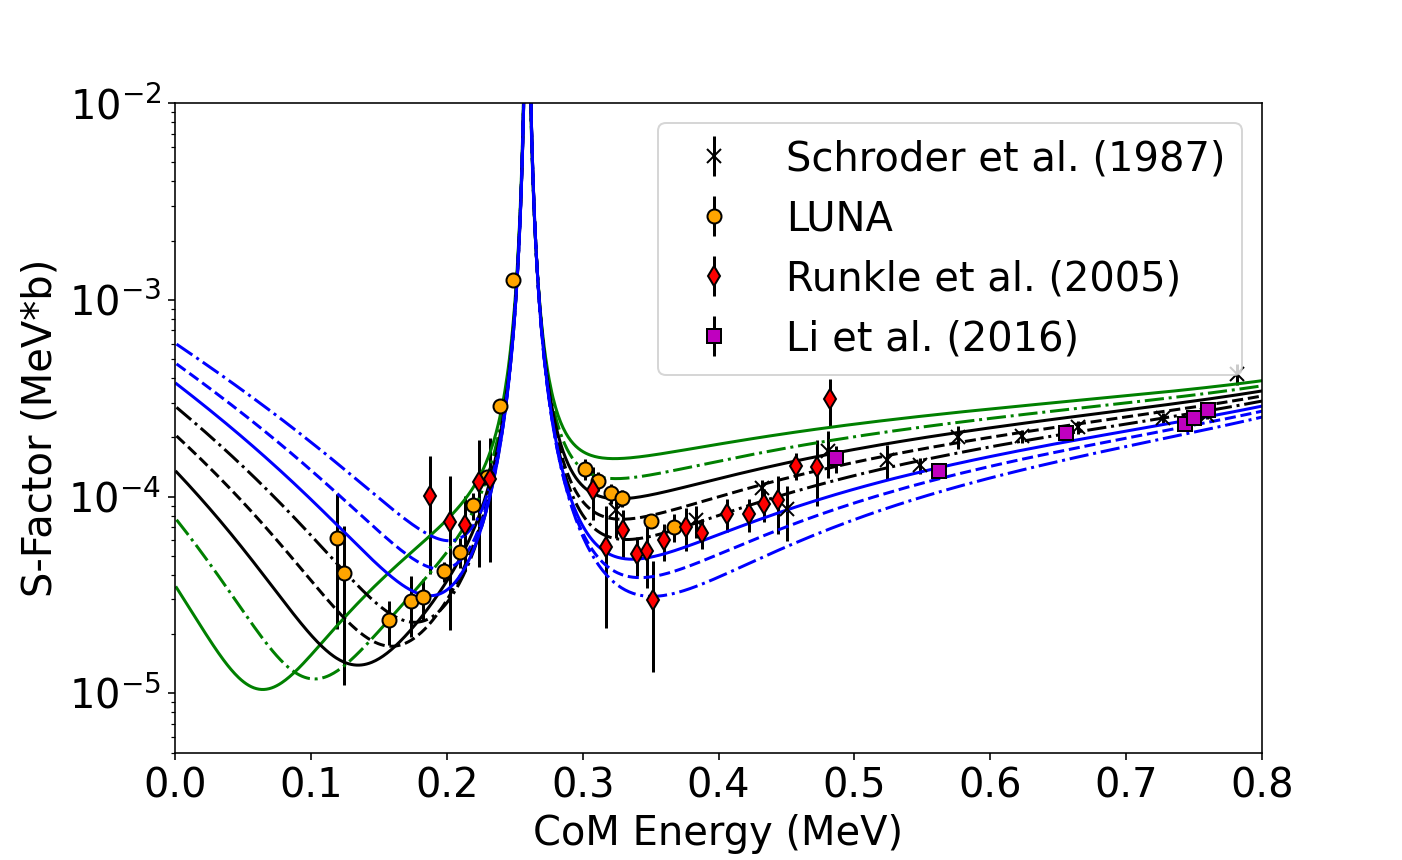
\includegraphics[width=1.0\linewidth]{./figures/lifetimeEffects.png}
\caption{$R$-Matrix fits exploring the uncertainty of our lifetime measurements to the low energy extrapolation. The width of the 6.79 MeV excited state in $^{15}$O is fixed during each fit and changed in each subsequent iteration to another value within our uncertainty range. This clearly shows that even though our lifetime result provides the most stringent limitation on the lifetime of this state, it still has an outsized effect on the low energy behavior of this reaction. The Schr{\"{o}}der et al.~data are from \cite{Schroder1987}, while the LUNA data represents the measurements \cite{Formicola2004, Imbriani2005, Marta2008, Marta2011}, the Runkle et al.~data are from \cite{Runkle2005}, and the Li et al.~data are from \cite{Li2016}. Of these, the data used from \citet{Li2016} are differential and were treated as such in the fitting but scaled up by 4$\pi$ for plotting purposes.}
\label{fig: rmatrixRange}
\end{figure}


\begin{figure}[h!]
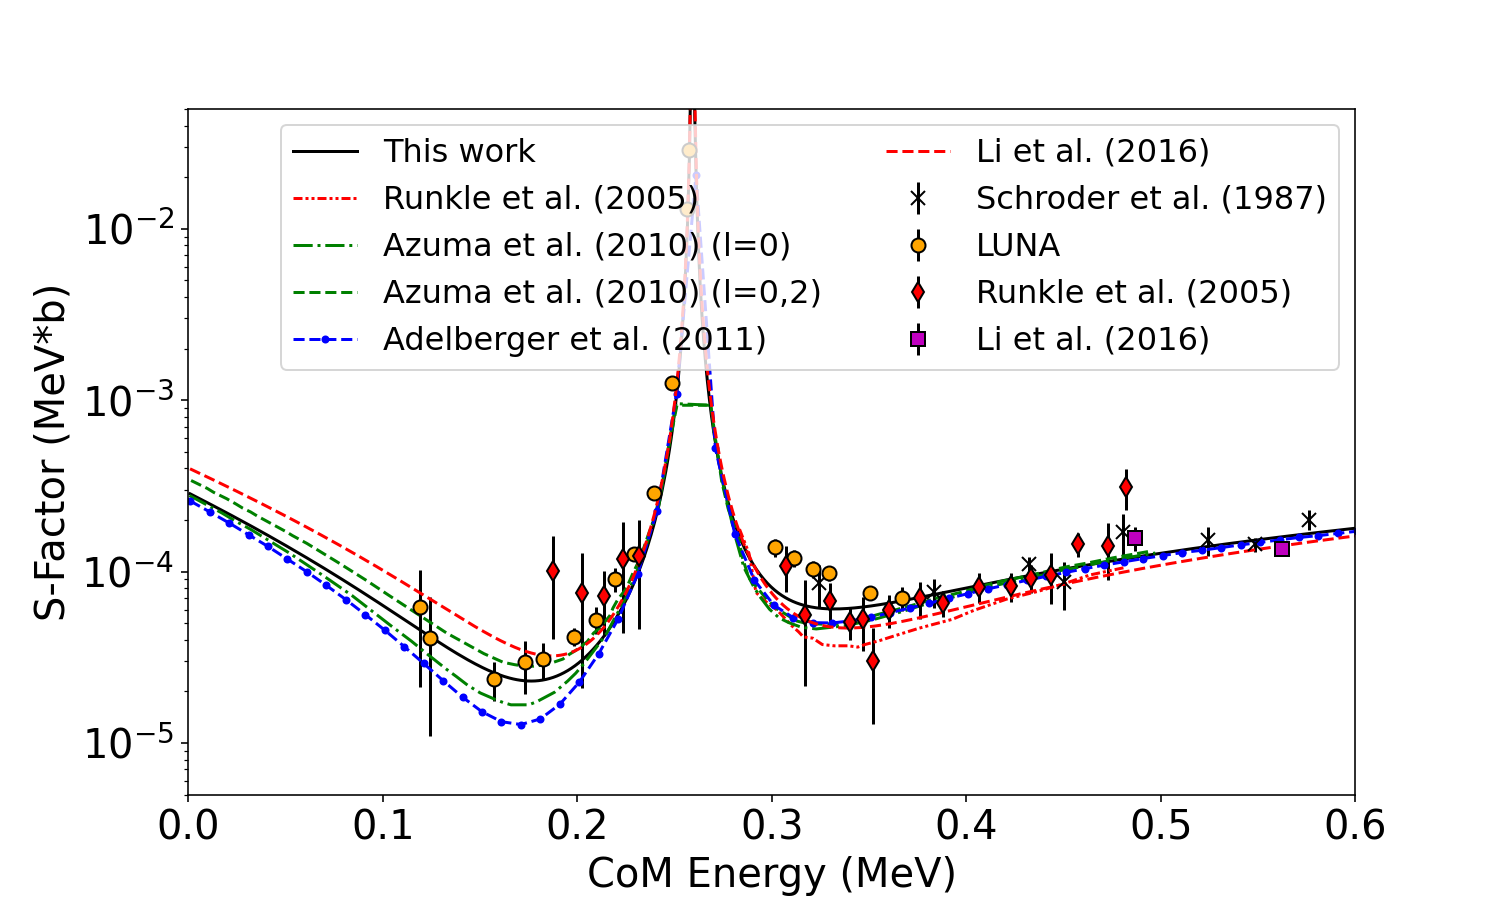
\includegraphics[width=1.0\linewidth]{./figures/bestFits.png}
\caption{$R$-matrix fits comparing our best fit with the lifetimes to those performed in previous works. Our fit used a lifetime value for the 6.79 MeV excited state in $^{15}$O within our measured range range, $\Gamma=2.75$ where the fits to the data provide good agreement with data above and below the 278 keV resonance. This plot is limited to the low energy region. The Schr{\"{o}}der et al.~data are from \cite{Schroder1987}, while the LUNA data represents the measurements of \cite{Formicola2004, Imbriani2005, Marta2008, Marta2011}, the Runkle et al.~data are from \cite{Runkle2005}, and the Li et al.~data are from \cite{Li2016}. Of these, the data used from \citet{Li2016} are differential and were treated as such in the fitting but scaled up by 4$\pi$ for plotting purposes. The fits from previous works come from Refs.~\cite{Runkle2005, Azuma2010, Adelberger2011, Li2016}.}
\label{fig: rmatrixClose}
\end{figure}

In examining the capture to the ground state in $^{15}$O, the $R$-matrix fits show the effect of our lifetime measurement. Specifically, in Fig.~\ref{fig: rmatrixRange}, we present fits showing the whole range of lifetimes for the 6.79 MeV state of $\tau = 0.6 \pm 0.4$. This shows that despite this measurement providing the most stringent limit on the lifetime, this range still translates into dramatic changes in the low energy behavior of the $S$-factor. Our fits, however, agree well with the capture data and previous studies. One of the best fits using our lifetimes is shown alongside fits from Refs.~\cite{Runkle2005, Azuma2010, Adelberger2011, Li2016} in Fig.~\ref{fig: rmatrixClose}. 

While the experimental results limit the previous uncertainty range in the lifetime data, this $R$-matrix analysis clearly demonstrates that it remains too large for solely reducing uncertainty in the extrapolation for the low energy range cross section of the ground state transition.




\section{Complete fit}
\label{sec: complete fit}


Beyond our new lifetime measurements, an $R$-matrix analysis was used to fit all the ground state and the 6.79 MeV transition differential cross section data measured in the current experiment, incorporating the new lifetimes, and an exhaustive set of previously measured data of the $^{14}$N$(p,\gamma)^{15}$O reaction.

Similar to the fits for examining the lifetime's effects, the information about the levels was obtained from \citet{Ajzenberg-Selove1991} or \citet{Daigle2016} where they had been updated. A channel radius of 5.5 fm was adopted for this work, which matches the analyses done by Refs.  \cite{Adelberger2011, Li2016, Wagner2018, Frentz2021}. Information about the levels and their parameters as used in \texttt{AZURE2} are contained in Table~\ref{table: fitParamsFullFit}. 


\begin{table*}[]
\thisfloatpagestyle{plain}
\caption{PARAMETERS USED IN THE FULL $R$-MATRIX FIT TO INCORPORATE THE CROSS SECTION DATA}
\begin{center}
\begin{threeparttable}
\begin{tabular}{c  c  c  c  c  c  c}
\toprule
$E_x$ (Ref.~\cite{Ajzenberg-Selove1991, Daigle2016}) &   $E_x$ (fit) & $J^\pi$ & Channel & l & s & ANC (fm$^{-1/2}$) / $\Gamma$ (eV)\\ 
\midrule
0.0 & 0.0	& 1/2$^-$ &	$^{14}$N+p &	1&	1/2&	{0.23}\\
	&	&	    &    $^{14}$N+p &	1&	3/2&	{7.4} \\
%5.183(1) & \textbf{5.183}&	1/2$^+$&	$^{14}$N+p&	0&	1/2&	\textbf{0.33}\\
%	&	&		    &$^{15}$O+$\gamma_{0.00}$  &	E1&	1/2&	\textbf{0.0784}\\
%5.2409(3) & \textbf{5.2409}&	5/2$^+$&	$^{14}$N+p &	2&	1/2&	\textbf{0.23}\\
%                &	&		  & $^{14}$N+p &	2&	3/2&	\textbf{0.24}\\
%	 			&	&	 &$^{15}$O+$\gamma_{0.00}$	&M2&	1/2&	\textbf{0.0002}\\
6.1763(17) & \textbf{6.1763}&	3/2$^-$& $^{14}$N+p &	1&	1/2&	{0.47}\\
				&	&	& $^{14}$N+p	&1	&3/2	&{0.53}\\
				&	&	&$^{15}$O+$\gamma_{0.00}$	&M1	&1/2&	\textbf{0.865}\\
6.7931(17) & {6.7931}&	3/2$^+$ & $^{14}$N+p &	0&	3/2&	{4.75}\\
	&	&	     &  $^{15}$O+$\gamma_{0.00}$	&  E1  &	1/2&	\textbf{2.50}\\
%	& &       &  $^{15}$O+$\gamma_{6.17}$	&  E1  &	3/2&{-0.002}\\
%6.8594(9) & \textbf{6.8594}&	5/2$^+$&	$^{14}$N+p&	2&	1/2&\textbf{0.39}\\
%	&		&    &     $^{14}$N+p&	2&	3/2&	\textbf{0.42}\\
%	&		&    &     $^{15}$O+$\gamma_{5.24}$&	M1&	5/2&	\textbf{0.04}\\
%7.2759(6) & \textbf{7.2759}&	7/2$^+$&	$^{14}$N+p &	2&	3/2&	\textbf{1541}\\
%	&		&    &     $^{15}$O+$\gamma_{5.24}$&	M1&	5/2&	\textbf{0.00099}\\
\hline
7.5565(4) & 7.5563	&	1/2$^+$	&	$^{14}$N+p	&	0	&	1/2	&	{1.0$\times$10$^3$}	\\
	&	&	&	$^{15}$O+$\gamma_{0.00}$	&	E1	&	1/2	&	\textbf{0.61$\times$10$^{-4}$}\\
	&	&	&	$^{15}$O+$\gamma_{6.79}$	&	M1	&	3/2	&	{8.22$\times$10$^{-3}$}\\
%	&	&	&	$^{15}$O+$\gamma_{5.18}$	&	M1	&	1/2	&	\textbf{0.006}\\
%	&	&	&	$^{15}$O+$\gamma_{6.17}$	&	E1	&	3/2	&	\textbf{0.0254}\\
8.2840(5)& \textbf{8.2848}&	3/2$^+$	&	$^{14}$N+p	&	2	&	1/2	&	\textbf{-92.2}\\
	&	&	&	$^{14}$N+p	&	0	&	3/2	&	\textbf{4.013$\times$10$^3$}\\
	&	&	&	$^{14}$N+p	&	2	&	3/2	&	\textbf{-509}\\
	&	&	&	$^{15}$O+$\gamma_{0.00}$	&	E1	&	1/2	&	\textbf{0.244}\\
%	&	&	&	$^{15}$O+$\gamma_{5.18}$	&	M1	&	1/2	&	{0.01}\\
%	&	&	&	$^{15}$O+$\gamma_{5.24}$	&	M1	&	5/2	&	{0.2}\\
%	&	&	&	$^{15}$O+$\gamma_{6.17}$	&	E1	&	3/2	&	{-4$\times$10$^{-3}$}\\
%	&	&	&	$^{15}$O+$\gamma_{6.86}$	&	M1	&	5/2	&	{0.01}\\
%8.743(6) & \textbf{8.7502}&	1/2$^+$	&	$^{14}$N+p	&	0	&	1/2	&	\textbf{35.726$\times$10$^3$}\\
%	&	&	&	$^{15}$O+$\gamma_{5.18}$	&	M1	&	1/2	&	\textbf{-0.2}\\
%	&	&	&	$^{15}$O+$\gamma_{6.17}$	&	E1	&	3/2	&	\textbf{0.0827}\\
%8.922(2) & \textbf{8.9219}&	5/2$^+$	&	$^{14}$N+p	&	2	&	3/2	&	\textbf{3.8$\times$10$^3$}\\
%	&	&	&	$^{15}$O+$\gamma_{6.79}$	&	M1	&	3/2	&	\textbf{0.003}\\
8.9821(17) & {8.98}&	5/2$^-$	&	$^{14}$N+p	&	1	&	3/2	&	{-5.872$\times$10$^3$}\\
	&	&	&	$^{15}$O+$\gamma_{0.00}$	&	E2	&	1/2	&	{-0.303}\\
	&	&	&	$^{15}$O+$\gamma_{6.79}$	&	E1	&	3/2	&	{-0.001}\\
9.484(8) & \textbf{9.488}&	3/2$^+$	&	$^{14}$N+p	&	2	&	1/2	&	\textbf{77.69$\times$10$^3$}	\\
	&	&	&	$^{14}$N+p	&	0	&	3/2	&	\textbf{126.685$\times$10$^3$}	\\
	&	&	&	$^{14}$N+p	&	2	&	3/2	&	\textbf{-7.822$\times$10$^3$}\\
	&	&	&	$^{15}$O+$\gamma_{0.00}$	&	E1	&	1/2	&	\textbf{6.92}\\
	&	&	&	$^{15}$O+$\gamma_{6.86}$	&	M1	&	5/2	&	{0.2}\\
9.488(3) & {9.4905}&	5/2$^-$	&	$^{14}$N+p	&	3	&	1/2	&	\textbf{0.979$\times$10$^3$}\\
	&	&	&	$^{14}$N+p	&	1	&	3/2	&	{-6.576$\times$10$^3$}\\
	&	&	&	$^{14}$N+p	&	3	&	3/2	&	{-0.985$\times$10$^3$}\\
	&	&	&	$^{15}$O+$\gamma_{0.00}$	&	E2	&	1/2	&	{-0.307}\\
	&	&	&	$^{15}$O+$\gamma_{6.79}$	&	E1	&	3/2	&	{-0.0123}\\
%9.609(2) & {9.6075}&	3/2$^-$	&	$^{14}$N+p	&	1	&	3/2	&	\textbf{-13.821$\times$10$^3$}\\
%	&	&	&	$^{15}$O+$\gamma_{0.00}$	&	M1	&	1/2	&	\textbf{1.24}\\
%     &	&	&	$^{15}$O+$\gamma_{6.79}$	&	E1	&	3/2	&	{-0.044}\\
%	&	&	&	$^{15}$O+$\gamma_{5.24}$	&	E1	&	5/2	&	{0.095}\\
%10.2817 & \textbf{10.2817}	&	5/2$^+$	&	$^{14}$N+p	&	2	&	3/2	&	\textbf{17.292$\times$10$^3$}\\
%	&	&	&	$^{15}$O+$\gamma_{6.79}$	&	M1	&	3/2	&	\textbf{0.2}\\	
%	&	&	&	$^{15}$O+$\gamma_{6.86}$	&	M1	&	5/2	&	\textbf{-0.4}\\	
%10.480 & \textbf{10.4675}	&	3/2$^-$	&	$^{14}$N+p	&	1	&	1/2	&	\textbf{28.998$\times$10$^3$}\\
%	&	&	&	$^{14}$N+p	&	1	&	3/2	&	\textbf{9.652$\times$10$^3$}\\
%	&	&	&	$^{15}$O+$\gamma_{0.00}$	&	M1	&	1/2	&	\textbf{-0.404}\\	
%	&	&	&	$^{15}$O+$\gamma_{6.79}$	&	E1	&	3/2	&	\textbf{0.1}\\
%	&	&	&	$^{15}$O+$\gamma_{6.86}$	&	E1	&	5/2	&	\textbf{0.1}\\
%10.506 & \textbf{10.5313}&	3/2$^+$	&	$^{14}$N+p	&	0	&	3/2	&	\textbf{205$\times$10$^3$}\\
%	&	&	&	$^{15}$O+$\gamma_{0.00}$	&	E1	&	1/2	&	\textbf{-0.195}\\
%	&	&	&	$^{15}$O+$\gamma_{6.79}$	&	M1	&	3/2	&	\textbf{0.3}\\
%	&	&	&	$^{15}$O+$\gamma_{6.86}$	&	M1	&	5/2	&	\textbf{-0.4}\\
%10.9288 & \textbf{10.9288}&	7/2$^+$	&	$^{14}$N+p	&	2	&	3/2	&	\textbf{56.948$\times$10$^3$}\\
%	&	&	&	$^{15}$O+$\gamma_{6.79}$	&	E2&	3/2	&	\textbf{1}\\
%11.218(3) & 11.217(2)& 3/2$^+$&	$^{14}$N+p	&	0	&	3/2	&	\textbf{40$\times$10$^3$}\\
%	&	&	&	$^{15}$O+$\gamma_{0.00}$	&	E1	&	1/2	& 5.21	\\   	
& {15}	&	1/2$^+$	&	$^{14}$N+p	&	0	&	3/2	&	{4.0$\times$10$^6$}\\
	&	&	&	$^{15}$O+$\gamma_{0.00}$	&	E1	&	1/2	&	\textbf{1.0$\times$10$^{3}$}	\\
& {15}	&	3/2$^+$	&	$^{14}$N+p	&	0	&	3/2	&	{4.722$\times$10$^6$}\\
	&	&	&	$^{15}$O+$\gamma_{0.00}$	&	E1	&	1/2	&	\textbf{327.3}	\\
%& \textbf{15}	&	5/2$^+$	&	$^{14}$N+p	&	2	&	1/2	&	\textbf{1.452$\times$10$^7$}\\
\bottomrule
\end{tabular}
\begin{tablenotes}
\small 
\item Levels used in the \textit{R}-matrix fits. Bold values indicate parameters which were allowed to vary during the fit. The signs on the partial widths and ANCs indicates the relative interferences. The dividing line demarcates the proton separation energy at $E_x$ = 7.2968(5) MeV \cite{Ajzenberg-Selove1991}. Levels where all parameters are fixed are not shown in this table for brevity but were included in the fits.
\end{tablenotes}
\end{threeparttable}
\label{table: fitParamsFullFit}
\end{center}
\end{table*}  


The cross-section data utilized in the fitting routine were from measurements at LUNA \cite{Formicola2004, Imbriani2005, Marta2008, Marta2011}, TUNL \cite{Runkle2005}, Bochum \cite{Schroder1987}, the University of Notre Dame \cite{Li2016}, and Dresden \cite{Wagner2018}. All of these data sets were left without scaling during the fits. The Bochum data from \citet{Schroder1987} were corrected as detailed in SFII \cite{Adelberger2011}. Due to target effects artificially inflating the cross section, we excluded some of the data from the fitting procedure close to sharp resonances. Corresponding to this, some of the resonance parameters were fixed in the fitting in order to enforce the known behavior of the resonances in the fit. 

Through our fitting process, we tested whether it was most appropriate to treat the various datasets as angle integrated or differential. For nearly all of the prior data, the original reported treatment was best. However, specifically for the data of \citet{Schroder1987}, by treating the dataset as differential in the fit instead of angle integrated, we dramatically improved our results, as evidenced by the reduction of 37$\%$ in the $\chi^{2}$ resulting from that change. Thus, our best fit from the data consisted of our measurements, \citet{Schroder1987}, and \citet{Li2016} as differential while the rest were treated angle integrated. These results can be seen in Figs.~\ref{fig: sfactor_best_fit} and \ref{fig: sfactor_best_low} and the final fit parameters are given in Table~\ref{table: fitParams}. 

\begin{figure}
\centering
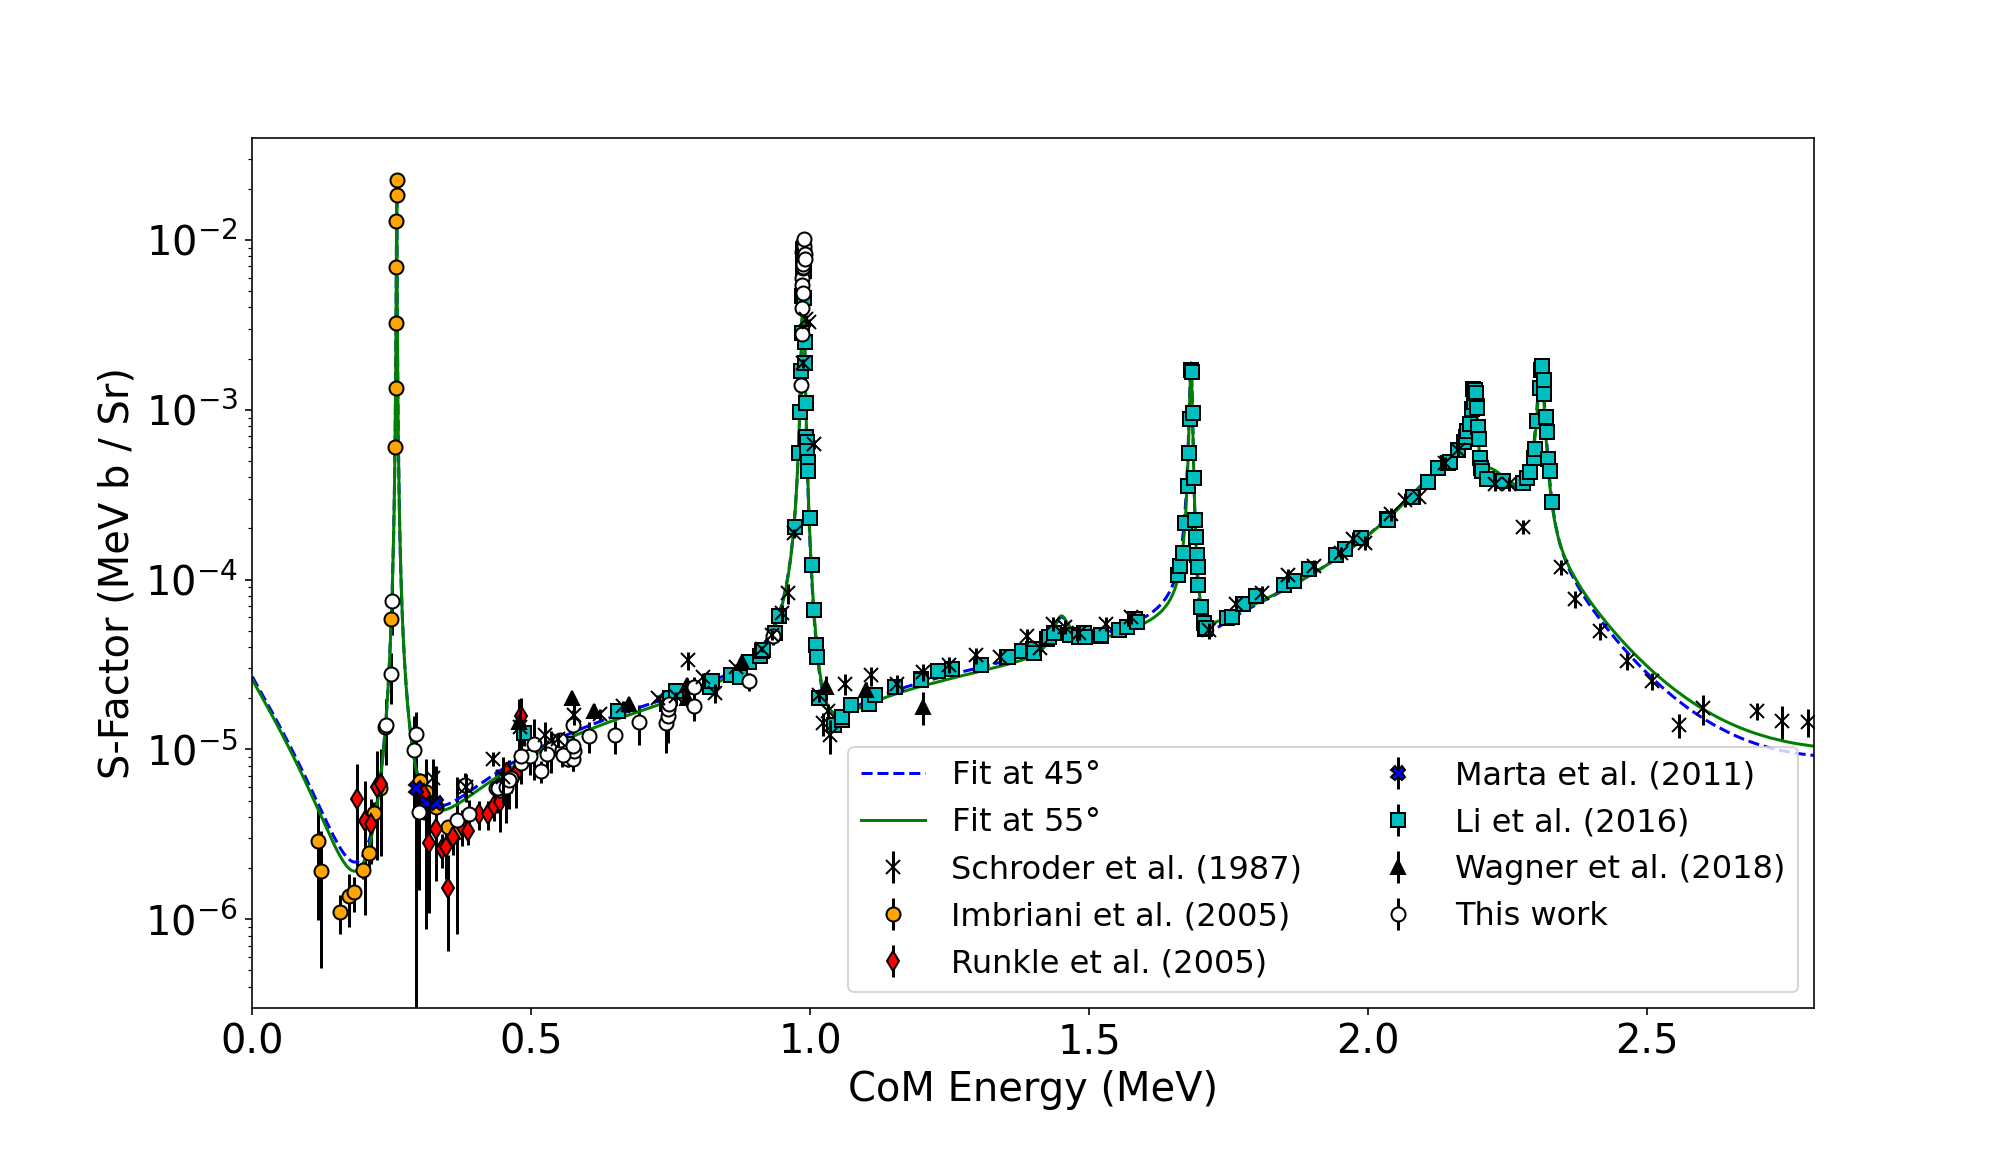
\includegraphics[width=1.0\columnwidth]{./figures/data_and_fits_whole.png}
\caption{$S$ factors for the R/DC $\rightarrow$ ground state transition for this work compared with those from Refs.~\cite{Imbriani2005, Marta2011, Runkle2005, Schroder1987, Li2016, Wagner2018} and extrapolated differential $S$-factor curves calculated with the \texttt{AZURE2} code. The data of \cite{Imbriani2005, Runkle2005, Marta2011, Wagner2018} have been scaled by a factor of $4\pi$ for the purposes of plotting the differential fits, but were treated an angle integrated when performing the fits. The data from \citet{Schroder1987} are corrected \cite{Adelberger2011} and then treated as differential (more detail in text). }
\label{fig: sfactor_best_fit}
\end{figure}

\begin{figure}
\centering
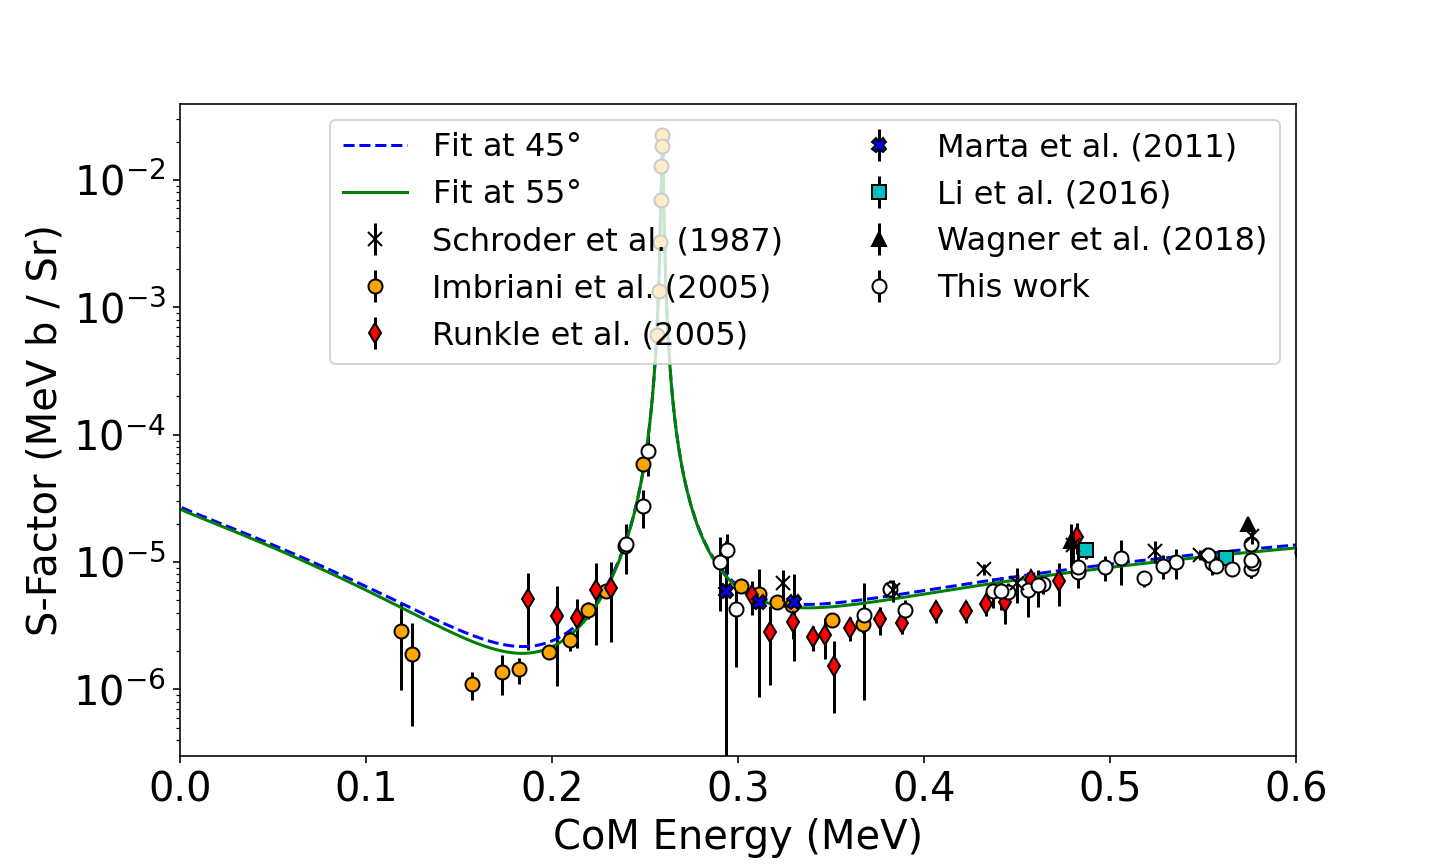
\includegraphics[width=1.0\columnwidth]{./figures/data_and_fits_low.png}
\caption{Low energy $S$-factor data and extrapolations for the R/DC $\rightarrow$ ground state transition for this work compared with those from Refs.~\cite{Imbriani2005, Marta2011, Runkle2005, Schroder1987, Li2016, Wagner2018} and extrapolated differential $S$-factor curves calculated with the \texttt{AZURE2} code. The data of \cite{Imbriani2005, Runkle2005, Marta2011, Wagner2018} have been scaled by a factor of $4\pi$ for the purposes of plotting the differential fits, but were treated an angle integrated when performing the fits. The data from \citet{Schroder1987} are corrected \cite{Adelberger2011} and then treated as differential (more detail in text). }
\label{fig: sfactor_best_low}
\end{figure}


Following this, we also examined the ways in which the differential cross section was affected by different angles. We calculated the differential $S$-factor at four different angles, namely $0\degree$, $45\degree$, $55\degree$, and $135\degree$, based on the results of our best fit to the data. As can be seen in Fig.~\ref{fig: sfactor_differential_angles}, there are significant differences in the differential $S$-factor across the entire energy landscape. Unsurprisingly, the fits at $45\degree$ and $55\degree$ are nearly identical. However, the fits at $0\degree$ and $135\degree$, surprisingly, exhibit the same behavior below the 278 keV resonance, and and are notably higher. They are elevated immediately below the resonance, and while the gap decreases with energy, the extrapolated $S_{g.s.}(0)$ for the fits at $0\degree$ and $135\degree$ are approximately 15$\%$ higher than the extrapolations at $45\degree$ and $55\degree$. Interestingly, while reported as angle integrated, the low-energy data of \citet{Imbriani2005} and \citet{Runkle2005} were measured at $55\degree$ and $0\degree$ respectively. As can be seen here, the discrepancy of these two data sets below the 278 keV resonance could be resolved in part by these angular differences. Specifically, a fit of these two datasets and the respective differential fits at $0\degree$ and $55\degree$ are shown in Fig.~\ref{fig: sfactor_runkle_imbriani}.

\textbf{Concluding sentence about this and how we handled it going forward.}


\begin{figure}
\centering
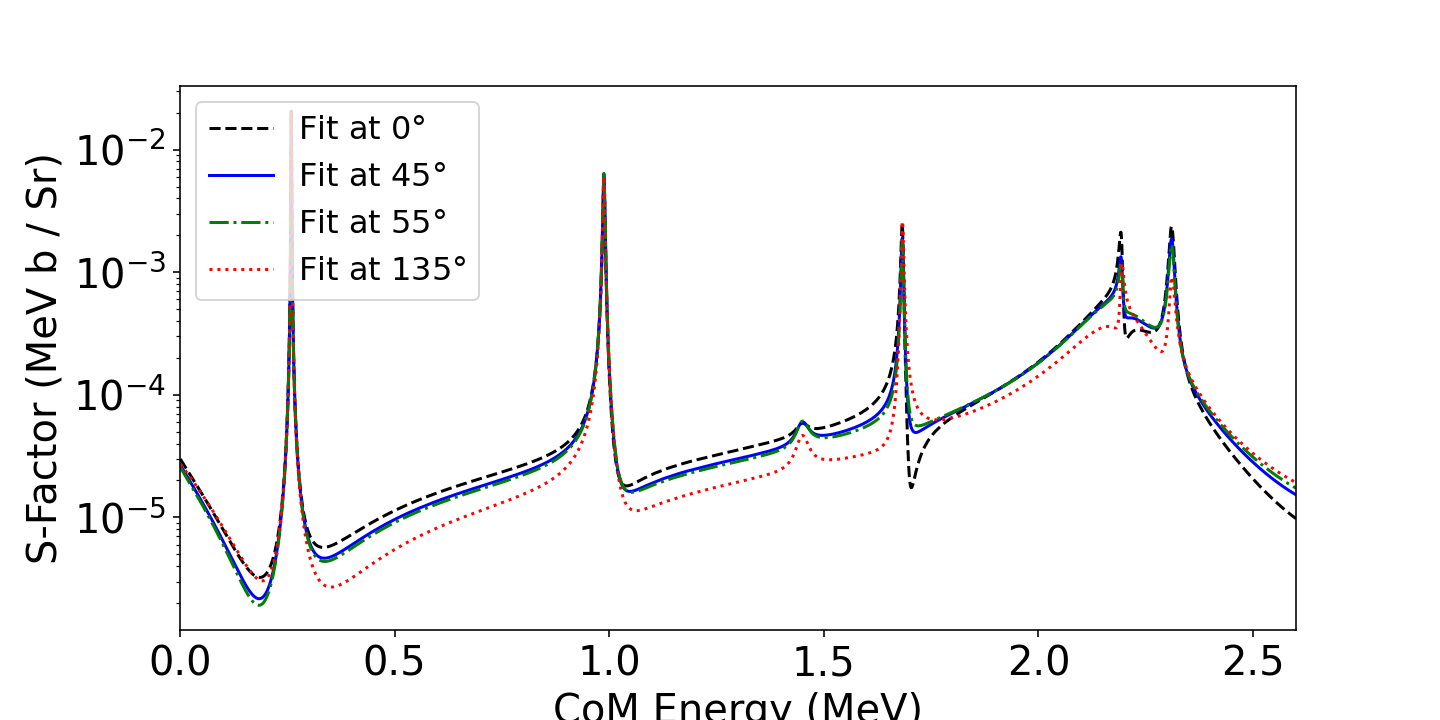
\includegraphics[width=1.0\columnwidth]{./figures/differential_fits.png}
\caption{Differential $S$ factors for the R/DC $\rightarrow$ ground state transition calculated from our best fit at $0\degree$, $45\degree$, $55\degree$, and $135\degree$. The behavior at different angles shows significant difference across the whole energy range for the reaction. }
\label{fig: sfactor_differential_angles}
\end{figure}

\begin{figure}
\centering
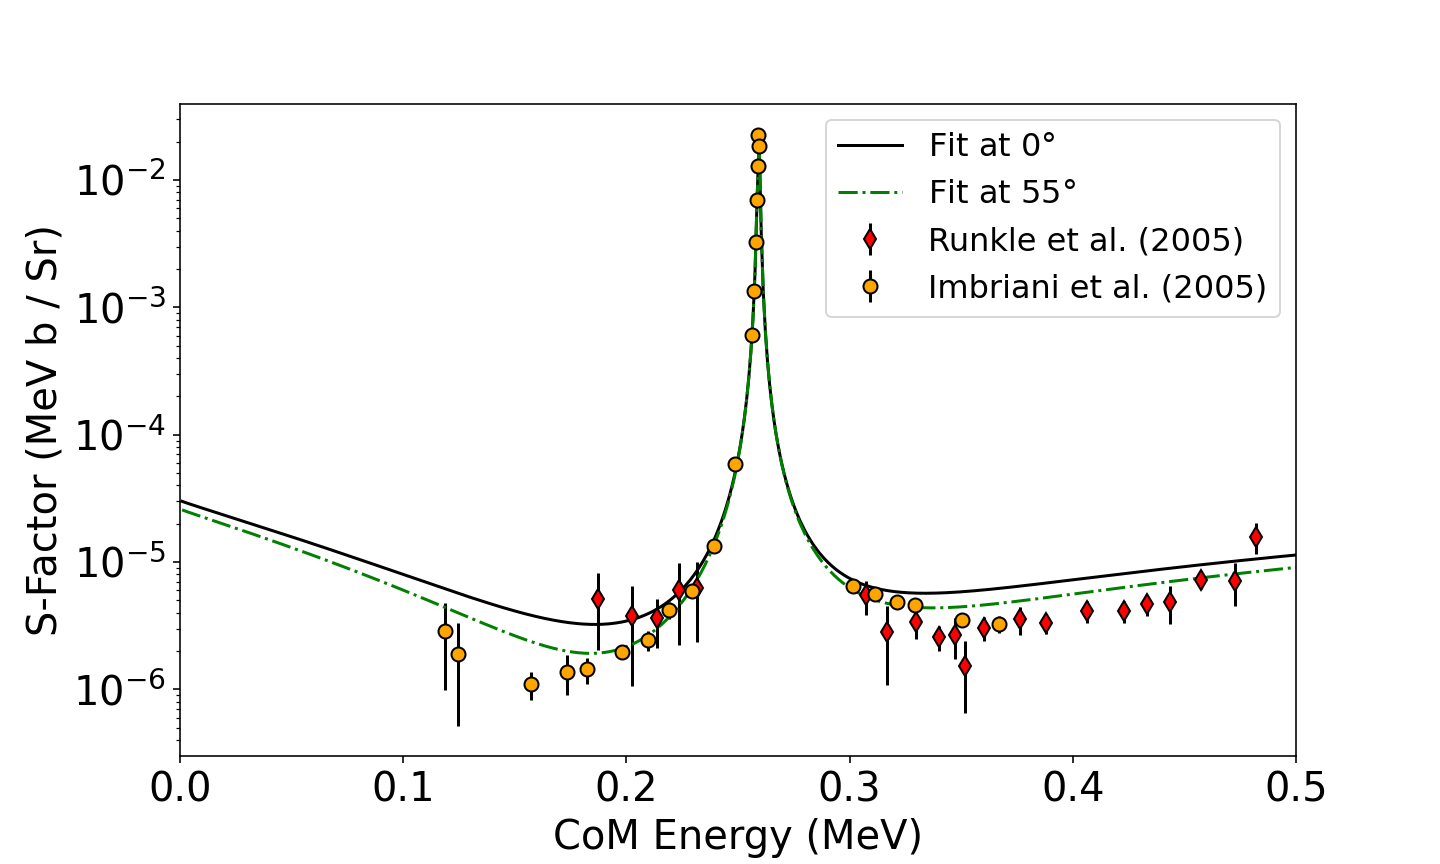
\includegraphics[width=1.0\columnwidth]{./figures/compare_runkle_imbriani.png}
\caption{$S$ factors for the R/DC $\rightarrow$ ground state transition from I\citet{Runkle2005} and \citet{Imbriani2005}, alongside the differential $S$-factors determined in this work at $0\degree$ and $55\degree$, respectively. The fits show signficant differences in the behavior of the reaction below the resonance, where the large discrepancy between these datasets lie. The data have been scaled by a factor of $4\pi$ for the purposes of comparing to the differential fits, but were treated an angle integrated when performing the fits. }
\label{fig: sfactor_runkle_imbriani}
\end{figure}


For the capture to the excited state at 6.79 MeV, the present fit is in agreement with earlier investigations. The present extrapolated $S$-factor for this transition is $S_{6.79}(0) = 1.24 \pm XX$ keV b. This agrees exactly with the recent measurement from \citet{Wagner2018} and simulataneously lies between the reports from \citet{Adelberger2011} and \citet{Li2016}, while agreeing with both. \textbf{I assume it will when the uncertainty is finished running anyway. }

For the capture to the ground state, the present result for the zero-energy extrapolated $S$-factor is $S_{g.s.}(0) = 0.33 \pm XX$ keV b. This value is higher than either that of \citet{Wagner2018} ($0.19 \pm 0.05$ keV b) and \citet{Adelberger2011} ($0.27 \pm 0.05$ keV b) while being lower than reported by \citet{Li2016} ($0.42 \pm 0.04$(stat)$^{+0.09}_{-0.19}$(syst) keV b). \textbf{Depending on our uncertainty, we will either agree or not with some of these or not. } 

\textbf{While we did not make any measurements for the transition to the excited state at 6.17 MeV, we included performed a fit and subsequent $S$-factor extrapolation using the data from \citet{Schroder1987}, \citet{Runkle2005}, and \citet{Imbriani2005}. The present extrapolated $S$-factor for this transition is $S_{6.17}(0) = 0.12 \pm XX$ keV b. Without any new data, this agrees well with the recently reported values of 0.12 by \citet{Azuma2010} and 0.13 $\pm$ 0.06 from \citet{Adelberger2011}.}

\textbf{Altogether, this allows us to assert a new total $S$-factor for the $^{14}$N$(p,\gamma)^{15}$O reaction. From this work, we find a total $S$-factor to be $S_{tot}(0) = 1.69 \pm XX$ keV b. This value, as well as those for the individual transitions can be seen compared to literature values in Table \ref{table: new_s_factors}.  The other transitions not explicitly reported in this section are expected to contribute approximately $\sim5\%$ to the total. Accounting for this, then, we expect the total $S$-factor to be inflated even more and have reflected that with an increased uncertainty.??} This total $S$-factor at zero-energy is higher than those values reported in \cite{Imbriani2005, Marta2008, Adelberger2011} but agrees reasonably well within uncertainty and lies in near perfect agreement to the extrapolations reported in \cite{Runkle2005, Angulo2005} but also agrees well within error. This suggests an enhancement in the low-energy behavior of the $^{14}$N$(p,\gamma)^{15}$O reaction, agreeing with the recent neutrino measurements by the Borexino group, reported in \citet{agostini2020direct}.


\begin{sidewaystable}[]
\caption{SUMMARY OF THE EXTRAPOLATED $S$-FACTORS}
\thisfloatpagestyle{plain}
\hspace*{-1.5cm}

\begin{threeparttable}
\begin{tabular}{@{}lllllll@{}}
\toprule
     &                                                          & \multicolumn{5}{c}{Astrophysical $S$-factor $S(0)$ (keV b)}                                                                                                                               \\ \midrule
Year & Reference                                                & R/DC $\rightarrow$ 0.00                         & R/DC $\rightarrow$ 6.79                 & R/DC $\rightarrow$ 6.17        & Others$^{d}$ & Total                                         \\
\hline
1987 & Schr{\"o}der \textit{et al.} \cite{Schroder1987}          & 1.55 $\pm$ 0.34                                 & 1.41 $\pm$ 0.02                         & 0.14 $\pm$ 0.05                & 0.1          & 3.20 $\pm$ 0.54                               \\
2001 & Angulo \textit{et al.}$^{a}$ \cite{Angulo2001}            & 0.08$^{+0.13}_{-0.06}$                          & 1.63 $\pm$ 0.17                         & 0.06$^{+0.01}_{-0.02}$          & $--$         & 1.77 $\pm$ 0.20                               \\
2003 & Mukhamedzhanov \textit{et al.} \cite{Mukhamedzhanov2003} & 0.15 $\pm$ 0.07                                 & 1.40 $\pm$ 0.20                         & 0.133 $\pm$ 0.02               & 0.02         & 1.70 $\pm$ 0.22                               \\
2004 & Formicola \textit{et al.} \cite{Formicola2004}            & 0.25 $\pm$ 0.06                                 & 1.35 $\pm$ 0.05 (stat) & 0.06$^{+0.01 \text{b}}_{-0.02}$ & 0.04         & 1.7 $\pm$ 0.1 (stat)        \\
 & & & $\pm$ 0.08 (sys) & & & $\pm$ 0.02 (sys) \\
2005 & Imbriani \textit{et al.} \cite{Imbriani2005}              & 0.25 $\pm$ 0.06                                 & 1.21 $\pm$ 0.05                         & 0.08 $\pm$ 0.03                & 0.07         & 1.61 $\pm$ 0.08                               \\
2005 & Runkle \textit{et al.} \cite{Runkle2005}                  & 0.49 $\pm$ 0.08                                 & 1.15 $\pm$ 0.05                         & 0.04 $\pm$ 0.01                & $--$         & 1.68 $\pm$ 0.09                               \\
2005 & Angulo \textit{et al.} \cite{Angulo2005}                  & 0.25 $\pm$ 0.08                                 & 1.35 $\pm$ 0.04                         & 0.06 $\pm$ 0.02                & 0.04         & 1.70 $\pm$ 0.07 (stat)       \\
 & & & & & & $\pm$ 0.10 (sys) \\
2006 & Bemmerer \textit{et al.} \cite{Bemmerer2006}              & $--$                                            & $--$                                    & $--$                           & $--$         & 1.74 $\pm$ 0.14 (stat)  \\
 & & & & & & $\pm$ 0.14 (sys)$^{c}$ \\
2008 & Marta \textit{et al.} \cite{Marta2008}                    & 0.20 $\pm$ 0.05                                 & $--$                                    & 0.09 $\pm$ 0.07                & $--$         & 1.57 $\pm$ 0.13                               \\
2010 & Azuma \textit{et al.} \cite{Azuma2010}                    & 0.28                                            & 1.3                                     & 0.12                           & 0.11         & 1.81                                          \\
2011 & Adelberger \textit{et al.} \cite{Adelberger2011}          & 0.27 $\pm$ 0.05                                 & 1.18 $\pm$ 0.05                         & 0.13 $\pm$ 0.06                & 0.08         & 1.66 $\pm$ 0.08                               \\
2016 & Li \textit{et al.} \cite{Li2016}                          & 0.42 $\pm$ 0.04 (stat)   & 1.29 $\pm$ 0.06 (stat)  & $--$                           & $--$         & $--$                                          \\
 & & $^{+0.09}_{-0.19}$(sys) & $\pm$ 0.06 (sys) & & & \\
2018 & Wagner \textit{et al.} \cite{Wagner2018}                  & 0.19 $\pm$ 0.01 (stat)          & 1.24 $\pm$ 0.02 (stat) & $--$                           & $--$         & $--$                                          \\
 & & $\pm$ 0.05 (sys) &  $\pm$ 0.11 (sys)  & & & \\ 
2021 & This work                  & 0.33 $\pm$ XX           & 1.24 $\pm$ XX  &  0.12  $\pm$ XX $^{d}$              & $--$         & 1.69 $\pm$ XX \\
 \bottomrule
\end{tabular}
\begin{tablenotes}
\small 
\item A summary of reported $S$-factors, including this work. a) $R$-matrix analysis on available data, not a measurement. b) Adopted from Angulo \textit{et al.} \cite{Angulo2001}. c) Measured $S$-factor at 70 keV. d) Calculated difference of the total $S(0)$ from the other transitions. d) Fit to the data of \cite{Schroder1987, Runkle2005, Imbriani2005} as no new data for this transition was measured.
\end{tablenotes}
\end{threeparttable}
\label{table: new_s_factors}
\end{sidewaystable}


% % uncomment the following lines,
% if using chapter-wise bibliography
%
% \bibliographystyle{ndnatbib}
% \bibliography{example}
